\documentclass[11pt]{article}

\newcommand{\cnum}{CM146}
\newcommand{\ced}{Fall 2017}
\newcommand{\ctitle}[3]{\title{\vspace{-0.5in}\cnum, \ced\\Problem Set #1: #2\\Due #3}}
\usepackage{enumitem}
\usepackage{graphicx}
\usepackage{amsmath}
\newcommand{\solution}[1]{{{\color{blue}{\bf Solution:} {#1}}}}
\usepackage[usenames,dvipsnames,svgnames,table,hyperref]{xcolor}

\renewcommand*{\theenumi}{\alph{enumi}}
\renewcommand*\labelenumi{(\theenumi)}
\renewcommand*{\theenumii}{\roman{enumii}}
\renewcommand*\labelenumii{\theenumii.}


\begin{document}
\ctitle{02}{Perceptron and Regression}{Feb 6,2018}
\author{}
\date{}
\maketitle
\vspace{-0.75in}

\section{Problem 1}
\begin{enumerate}
\item Two possible lines: $y = X_1 + X_2 - 2.1$,
  $y = X_1 + X_2 - 2.2$.
  \vspace{10}
\item XOR is not going to be linearly separable. This is because the convex
  hulls of data points that map to $0$ and to $1$ intersect.
\end{enumerate}

\newpage
\section{Problem 2}

\begin{enumerate}
\item
  \begin{align*}
    \frac{\partial J}{\partial \theta_j}
    &=
    -\sum_{n=1}^N \left[y_n \frac{x_j}{h_{\theta}(\textbf{x}_n)}
      + (y_n-1)\frac{x_j}{1-h_{\theta}(\textbf{x}_n)}\right]\\
    &= \frac{y_n - h_\theta(\textbf{x}_n)}{h_\theta (\textbf{x}_n) [1 - h_\theta(\textbf{x}_n)]}x_j
  \end{align*}
\end{enumerate}
\newpage
\section{Problem 3}
\begin{enumerate}
\item
    \begin{align*}
    \frac{\partial J}{\partial \theta_0}
    &=
    \sum_{n=1}^N 2(\theta_0 + \theta_1 \textbf{x}_{n,1} - y_n)w_n
    \end{align*}
    \begin{align*}
      \frac{\partial J}{\partial \theta_1}
    &=
      \sum_{n=1}^N 2(\theta_0 + \theta_1 \textbf{x}_{n,1} - y_n)w_n\textbf{x}_{n,1}
    \end{align*}
  \item
    Define the following:
    \begin{align*}
      \textbf{W} &= \begin{bmatrix}
        w_1 &\dots &0\\
        \vdots &\ddots &0\\
        0 &\dots &w_N\\
      \end{bmatrix}\\
        \textbf{X} &= \begin{bmatrix}
          1 &x_{1,1}\\
          1 &x_{2,1}\\
          \vdots &\vdots\\
          1 &x_{N,1} 
        \end{bmatrix}\\
        \textbf{Y} &= \begin{bmatrix}
          y_1\\
          y_2\\
          \vdots\\
          y_N
        \end{bmatrix}\\
        \theta &= \begin{bmatrix}
          \theta_0\\
          \theta_1
        \end{bmatrix}
    \end{align*}
    We know that (adding $1/2$ for conveniance):
    \begin{align*}
      J(\theta)
      &= \frac{1}{2}(\textbf{X}\theta - \textbf{Y})^T\textbf{W}(\textbf{X}\theta - \textbf{Y}).\\
      \frac{\partial}{\partial \theta} J(\theta) &= \frac{1}{2}(\textbf{X}\theta - \textbf{Y})^T\textbf{W}(\textbf{X}\theta - \textbf{Y}).\\
      &= \frac{1}{2}\frac{\partial}{\partial \theta}(\theta^T\textbf{X}^T\textbf{W}\textbf{X}\theta - \theta^T\textbf{X}^T\textbf{W}\textbf{Y} - \textbf{Y}^T\textbf{W}\textbf{X}\theta + \textbf{Y}^T\textbf{W}\textbf{Y})\\
      &= \textbf{X}^T\textbf{W}\textbf{X}\theta - \textbf{X}^T\textbf{W}\textbf{Y}
    \end{align*}
    To minimize we need $\textbf{X}^T\textbf{W}\textbf{X}\theta - \textbf{X}^T\textbf{W}\textbf{Y} = 0$. This gives us
    \begin{equation*}
      \theta = (\textbf{X}^T\textbf{W}\textbf{X})^{-1}\textbf{X}^T\textbf{W}\textbf{Y}.
    \end{equation*}
\end{enumerate}
\section{Problem 4}
\begin{enumerate}
\item Since data is linearly separable, we know that there exists $\vec{w}$
  such that for all $(\vec{x}_i, y_i)$:
  \begin{equation*}
    y_i = \begin{cases}
      1, \quad \vec{w}^T\vec{x}_i + \theta \geq 0\\
      -1, \quad \vec{w}^T\vec{x}_i + \theta < 0.
    \end{cases}
  \end{equation*}
  So, we know that $y_i(\vec{w}^T\vec{x}_i + \theta) > 0$. Let the minimum of
  all of these be for $j$ and let
  $y_j(\vec{w}^T\vec{x}_j + \theta) = \eta > 0$. Now pick
  $\hat{w} = w\eta^{-1}$ and $\hat{\theta} = \theta \eta^{-1}$. Notice that
  $\hat{w}$ and $\hat{\eta}$ give $\delta = 0$.
\item If there is an optimal solution $\vec{w}$, $\theta$ with $\delta = 0$
  that implies that for all $(\vec{x}_i, y_i)$
  \begin{equation*}
    y_i(\vec{w}^T\vec{x}_i + \theta) \geq 1
  \end{equation*}
  Which implies that, due to the fact that $\vec{w}^T\vec{x}_i + \theta$
  and $y_i$ have the same sign, for all $(\vec{x}_i, y_i)$
  \begin{equation*}
    y_i = \begin{cases}
      1, \quad \vec{w}^T\vec{x}_i + \theta \geq 0\\
      -1, \quad \vec{w}^T\vec{x}_i + \theta < 0.
    \end{cases}
  \end{equation*}
  which implies linear separability by definition.
\item Depends for which value of $\delta$ the hyperplane generates. If
  $\delta < 1$, i.e. $1-\delta > 0$, the problem boils down to the above case
  and the data is linearly separable. However, if $\delta > 1$ that means that
  $1-\delta < 0$, which means there is no gurantee that
  $\vec{w}^T\vec{x}_i + \theta$ and $y_i$ will have the same sign, which
  implies we cannot infer anything about linear separability and that the given
  plane does not separate the data.
\item Take $\theta = 0$, $w^T = \begin{bmatrix} 0 &0 &0 \end{bmatrix}$, and
  we will have $\delta = 0$, which is optimal due to the constraint
  $\delta \geq 0$.
\item Take $\theta = 0$, $w^T = \begin{bmatrix} 1 &1 &1\end{bmatrix}$.
\end{enumerate}
\newpage
\section{Problem 5}
\begin{enumerate}
\item The test data seems to intuitively match the best fit polynomial of the training data.
  The training data seems to be fitted best by a polynomial of degree three. Both the training
  and test data have a relatively high amount variance, but these two variances are similar
  to eachother. Particularly, the data seems to deviate from a degree three polynomial with a
  normal distribution.
    \begin{figure}[h]
      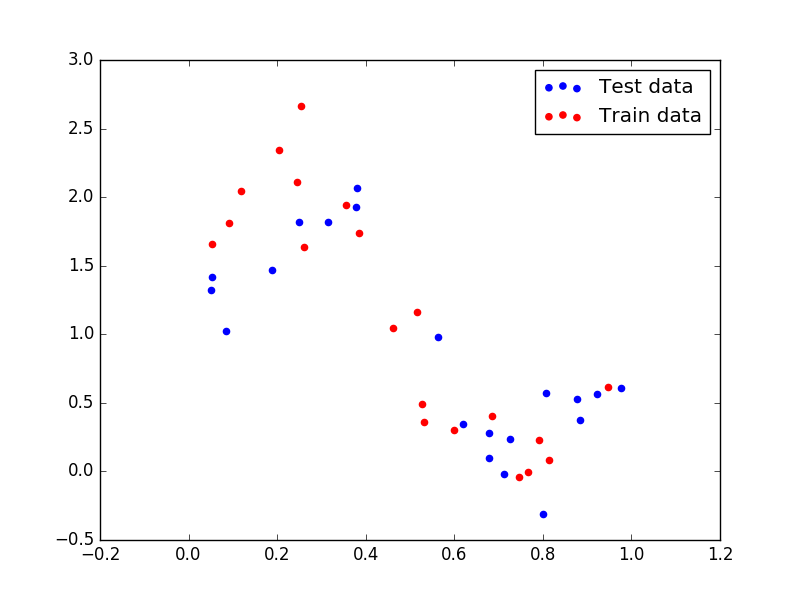
\includegraphics[height=10cm]{data.png}
    \end{figure}  
\item
\item
\item
  \begin{tabular}{ c | c | c | c | c }
    Learning rate & Iterations & Coeficients & Train Cost & Test Cost \\
    10^{-2} & 764 & [2.4464, -2.8163] & 3.9126 & 7.047 \\
    10^{-3} & 7020 & [2.4464, -2.8163] & 3.9126 & 7.047 \\
    10^{-4} & 10000 & [2.27044, -2.4606] & 4.086 & 5.841 \\
    0.0407 & 10000 & [-9\times10^{18}, -4\times10^{18}] & 2\times 10^{39} & 2 \times 10^{39}
  \end{tabular}
\item A closed-form solution in this context means that there is an explicit
  way to exactly calculate the optimal value (assuming mean-square error) of
  weights by just multiplying and adding known values.

  The train, test costs and the coefficients match exactly to the gradient
  descent fit where $\eta = 0.01$ (probably not exactly, but close enough
  for me not to be able to see the difference in python's float
  representation).
\item
    \begin{tabular}{ c | c | c | c }
      Iterations & Coeficients & Train Cost & Test Cost \\
      1356 & [2.4464, -2.81635] & 3.9126 & 7.047
  \end{tabular}
  \item
  \item RMSE is a better metric here because the error will have the same
    dimensionality as the actual distance between predicted and true values.
    Therefore, RMSE will provide a more linear comparison of quality. This
    means that if RMSE is twice as bad, we can say that the model sort of
    predicts twice as bad, while saying this for $J(\theta)$ would certainly
    be incorrect.
  \item The best polynomial is probably of degree $3$, since it provides the
    lowest RMS error, while also being less complex than other models that
    have similar test data performance ($4$, $5$, $6$, $7$). There is evidence
    of overfitting for $m>8$. Here we see that the training data is being
    fitted better and better, yet the test data becomes very bad very fast.
    Also, the data is underfitted for $m=0$, since the test data performs
    better than the training data for this case.
    \begin{figure}[h]
      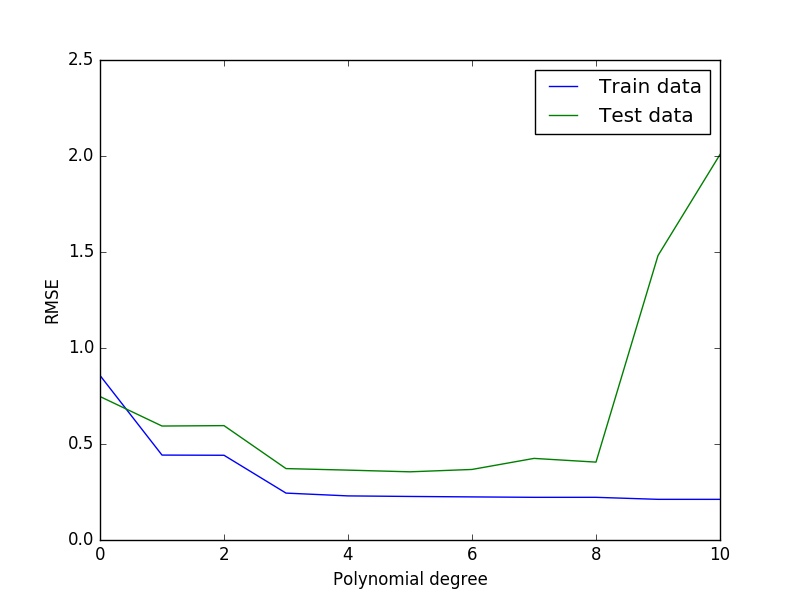
\includegraphics[height=10cm]{fig1.png}
    \end{figure}
\end{enumerate}
\end{document}
